\documentclass[a4paper]{article}

%% Language and font encodings
\usepackage[english]{babel}
\usepackage[utf8x]{inputenc}
\usepackage[T1]{fontenc}

%% Sets page size and margins
\usepackage[a4paper,top=3cm,bottom=2cm,left=3cm,right=3cm,marginparwidth=1.75cm]{geometry}

%% Useful packages
\usepackage{amsmath}
\usepackage{graphicx}
\usepackage[colorinlistoftodos]{todonotes}
\usepackage[colorlinks=true, allcolors=blue]{hyperref}

\usepackage{caption}
\usepackage{subcaption}

\graphicspath{{res/}}

\title{Your Paper}
\author{Lukas Finkbeiner}

\begin{document}
\maketitle

\begin{abstract}

We studied signals.

\end{abstract}

% No need to re-derive anything!!

\section{Introduction and Background}

\subsection{The Fourier Transform}

Where $V(t)$ is voltage as a function of time and $V(\nu)$ is voltage as a function of frequency $\nu$.

\

$V(\nu) = \int_{-T / 2}^{T / 2} V(t) \exp(2 \pi i \nu t) dt$

\

Where T is the length of the time sample.

\

$V(t) = \frac{1}{\nu_s} \int_{- \nu_s / 2}^{\nu_s / 2} \tilde{V}(\nu) \exp(-2 \pi i \nu t) d \nu$

\

where $\nu_s$ is the sampling frequency used.

\textcolor{red}{What happens if you change the bounds in the manner (N / 2 - 1) / $\nu_s$}

% ?? I need to talk about Parseval's Theorem

\subsection{Positive and Negative Frequencies}

``complex inputs to a Fourier Transform break the positive/negative frequency degeneracy''

The sine function is odd:

$\sin(-\omega t) = -sin(\omega t)$

The cosine function is even:

$\cos(-\omega t) = \cos (\omega t)$

We can generalize under Euler's identity:

$A\exp(i \omega t) = A \cos(\omega t) + i \cdot A \sin(\omega t)$

$A\exp(-i \omega t) = A \cos(-\omega t) + i \cdot A \sin(-\omega t) = A \cos(\omega t) - i \cdot A \sin(\omega t)$

\textcolor{red}{Show how such a formulation can explain a phase shift.}

\subsection{Nyquist's Theorem and Aliasing}

$f_s > 2 f_{max}$

\subsection{The Convolution and Correlation Theorems}

The convolution of two functions $f(t)$ and $g(t)$ is defined as:

\

$[f * g](\tau) = \int_{-T / 2}^{T / 2} f(t) g(\tau - t) dt$

\

The correlation of two functions $f(t)$ and $g(t)$ is defined as

\

$[f \star g](\tau) = \int_{-T / 2}^{T / 2} f(t) g(\tau + t) dt$

\

\textcolor{red}{You may want to prove this by substituting the Fourier transform}

\

$[\tilde{f * g}](\nu) \equiv \int_{-T / 2}^{T / 2}[f * g](\tau) \exp{2 \pi i \tau \nu} d \tau = \tilde{f}(\nu) \cdot \tilde{g}(\nu)$

\

$[\tilde{f \star g}](\nu) \equiv \int_{-T / 2}^{T / 2}[f \star g](\tau) \exp{2 \pi i \tau \nu} d \tau = \tilde{f}(\nu) \cdot \tilde{g^*}(\nu)$

\textcolor{red}{Now: how is the ACF relevant to this paper}

\subsection{Sideband Theory}

All that sweet, sweet trig.

\section{Methods}

\quad \quad This is the equipment I used. These are the libraries and functions I used. This is how I used them ($vague$ hint at your code). Uncertainty? Technical errors?

\

To begin our investigation of the Nyquist criterion, we decided on a sampling frequency $\nu_s = 6.25$ MHz at which the pico sampler (a PicoScope 2206A) remained for the duration of the data collection for all signals. We then used the N9310A RF Signal Generator to output signals at frequency $\nu_0$: fractions of the sampling frequency. For example, one of our input signals was $\nu_0 = .4 \nu_s = 2.5$ MHz. For all signals, we performed visual inspections of the pico sampler's input by using a T-joint and connecting the output to an oscilloscope (a Rigol DS1052E). We used the ugradio module to perform data collection (ugradio.pico.capture\_data) and, later on, to perform Fourier and inverse Fourier transforms (ugradio.dft.dft and ugradio.dft.idft).

To consider the frequency resolution for two signals of similar frequency, we employed a second signal generator. The 83712B has a lower limit of 10 MHz output frequency. Consequently, we set our original signal generator to small increments above that frequency and needed to increase the sampling frequency to $\nu_s = 31.25$ MHz.

To investigate the impact of noise on the Fourier transform, we switched the pico sampler's input to an NOD 5250 noise generator (6 MHz bandpass) at zero attenuation. We collected 32 blocks of 16000 samples from the PicoScope, this time using the sampling frequency $\nu_s = 62.5$ MHz.

We explored mixers and sideband theory with a Mini-Circuits ZAD-1. We the 83712B as the local oscillator and the N9310A as the RF input. We sent the output to the oscilloscope and PicoScope, this time using a $50 \Omega$ terminator to eliminate bounce-back interference. The ZAD-1 works best for signals above 10 MHz, so we set the local oscillator to $\nu_{LO} = 11$ MHz and collected two sets of data: one for which $\nu_{RF} = 11.55$ MHz and one for which $\nu_{RF}=10.45$ MHz (thus, $\Delta \nu = .05 \nu_{LO} = .55$ MHz. 

The mixed signals were somewhat weak, so we used 1.5 dBm amplitudes on both signal generators. We again used a sampling frequency of $\nu_s = 62.5$ MHz, motivated by the following identities:

$\sin(\nu_{LO}) \sin(\nu_{LO} + \Delta \nu) = \frac{1}{2} (\cos \Delta \nu - \cos (2\nu_{LO} + \Delta \nu))$ by evenness of the cosine function

and

$\sin(\nu_{LO}) \sin(\nu_{LO} - \Delta \nu) = \frac{1}{2} (\cos \Delta \nu - \cos (2\nu_{LO} - \Delta \nu))$

Now, if we expect to see two signals, $2\nu_{LO} + \Delta \nu = 23.1$ 23.1 is the highest frequency that we would expect. Our PicoScope offers sampling rates by dividing the base $62.5$ MHz. 31.25 MHz would have failed the Nyquist criterion, so we used the maximum sampling rate instead. 

Finally, we constructed a single-sideband mixer by using two mixers. Both mixers used both the local oscillator and radio frequency signals, but one of the mixers' RF input was phase shifted by approximately $\pi / 2$ by linking smaller cables together until we roughly satisfied the $\lambda / 4$ criterion.

\textcolor{red}{I don't remember the model of the other mixer} 

\section{Notes to Self}

% I could try zeroing out the different averages again. Maybe the log plot would look nicer. But you couldn't just use zeroes, becaus on a log plot that just creates a spike in the opposite direction.

What am I doing? Not ACF (5.3, 5.7) and procrastinating on 5.5 so that I can get some writing done.

\textcolor{red}{I did ACF analysis for neither 5.3 nor 5.7}

\textcolor{red}{Major logic error: side-by-side captions are mutilated!}

\textcolor{green}{Idea: put signal and power spectrum plots side by side, not signals with signals}

%\textcolor{black}


argue what the Nyquist criterion is, based on results.

* Include make and model of all equipment used.

* "Don't quote a number without the uncertainty and units."

% ?? is now the code I use to point out areas to which I need to return later.

Discussion on results for week 2, section 1

\

I need to include details about the equipment used, but how in-depth do I need to go? Current plan

* For most things, use model number and manufacturer

* When data analysis depends on a spec sheet, offer a brief summary of the specs to which you are referring to fine-tune your analysis

\

\textcolor{red}{I need uncertainties on results but I do not yet know how to get these.}

Closer to the end of writing, design a new subsection layout for the results section. You of course cannot make references like ``5.2'' and ``7.3'' in the submission.

\section{Results}

\subsection{5.2}

\quad \quad We took the default 16000 samples for each of our first signal samples. However, for the data analysis, we will be excluding the first 100 samples due to a peculiarity of the pico sampler which distorted these (see figure \ref{fig:pico_start}).

% Perhaps not important to discuss differences in peak to peak voltages across trials

\begin{figure}
\centering
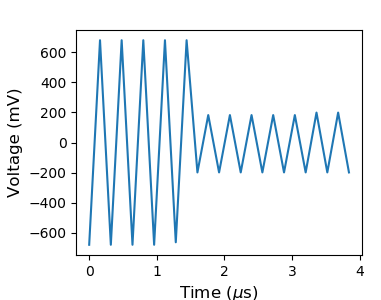
\includegraphics[width=0.5\textwidth]{5-2/pico_bad}
\caption{The oscilloscope displayed a constant signal throughout the period of data-taking. The data sampled from the pico sampler, however, reconstructs a signal with large aberrations in the first few microseconds.}
\label{fig:pico_start}
\end{figure}

\begin{figure}
\centering
\begin{minipage}{.5\textwidth}
	\centering
	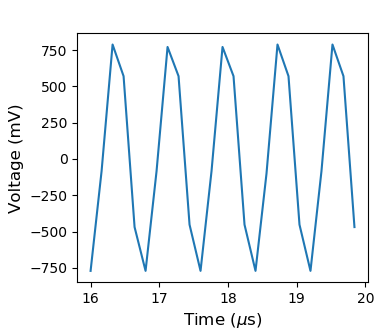
\includegraphics[width=.8\linewidth]{5-2/trial2}
	\caption{$\nu_0 = .2 \nu_s = 1.25$ MHz.}
	\label{fig:Nyq2}
\end{minipage}%
\begin{minipage}{.5\textwidth}
	\centering
	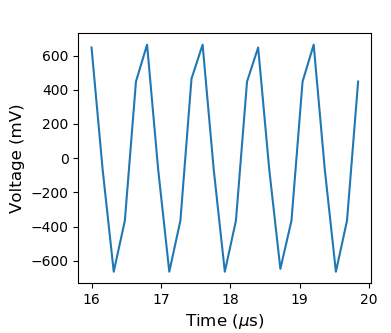
\includegraphics[width=.8\linewidth]{5-2/trial8}
	\caption{$\nu_0 = .8 \nu_s = 5$ MHz.}
	\label{fig:Nyq8}
\end{minipage}
\end{figure}

\begin{figure}
\centering
\begin{minipage}{.5\textwidth}
	\centering
	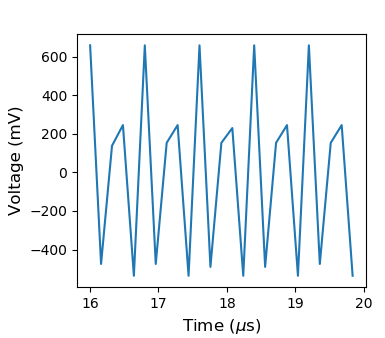
\includegraphics[width=.8\linewidth]{5-2/trial4}
	\caption{$\nu_0 = .4 \nu_s = 2.5$ MHz.}
	\label{fig:Nyq4}
\end{minipage}%
\begin{minipage}{.5\textwidth}
	\centering
	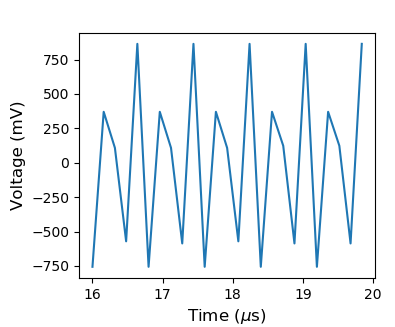
\includegraphics[width=.8\linewidth]{5-2/trial6}
	\caption{$\nu_0 = .6 \nu_s = 3.75$ MHz.}
	\label{fig:Nyq6}
\end{minipage}
\end{figure}
	
We may begin inspection of the samples with a qualitative approach. Figure \ref{fig:Nyq2} shows a signal which repeats about five times in the span of about 4 microseconds. This gives us 1.25 cycles per microsecond, or 1.25 MHz, as expected. Figure \ref{fig:Nyq8} still appoars as a sine wave, but visual inspection is no longer reliable. Again: we see about 5 samples in the span of about 4 microseconds. This would give 1.25 MHz, but because we know that our input signal was in fact $\nu_0 = 5$ MHz, we know that the waveform is aliased.

A more nuanced example comes from frequencies close to $.5 \nu_s$: compare figures \ref{fig:Nyq4} and \ref{fig:NyPw6}. Keeping in mind that only the frequency varied between trials and not the shape of the signal, a visual inspection is now confused: the sample looks like a sine wave in neither case. If take for granted that \ref{fig:Nyq4} is not a perfect sample, we may still visually estimate the frequency by noting 10 pairs of relative extrema (2.5 MHz). 

% ?? Maybe I should put these annotations in the captions (it would be more appropriate there, I think)

% ?? These figures need annotations. You can probably just do the same qualitative thing that you did before.

The power spectra exactly confirm these estimations. Furthermore, there are no obvious aberrations in the power spectra to indicate whether the signal was aliased during sampling. Consider, for example, that figures \ref{fig:NyPw4} and \ref{fig:NyPw6} are identical. An argmax function yielded precisely the same values for the frequency peaks.

The power spectrum for our fifth trial ($\nu_0 = .5 \nu_s = 3.125$ MHz) yielded an argmax with many digits (all other power spectra, even the aliased, returned frequencies to two decimal places). In other words, the calculation becomes more sensitive in a small region around this midpoint. All frequencies above this returned incorrect maxima in the power spectrum, so we have verified the Nyquist criterion. 

\textcolor{red}{?? No value and no uncertainty for this trial}

\begin{figure}
\centering
\begin{minipage}{.5\textwidth}
	\centering
	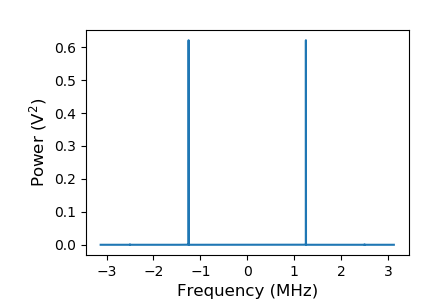
\includegraphics[width=.8\linewidth]{5-2/pow2}
	\caption{$\nu_0 = .2 \nu_s = 1.25$ MHz. Peak amplitudes at $\pm$ 1.25 MHz}
	\label{fig:NyPw2}
\end{minipage}%
\begin{minipage}{.5\textwidth}
	\centering
	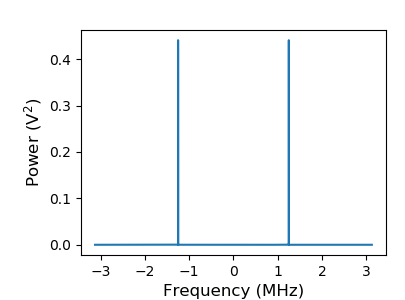
\includegraphics[width=.8\linewidth]{5-2/pow8}
	\caption{$\nu_0 = .8 \nu_s = 5$ MHz. Peak amplitudes at $\pm$ 1.25 MHz}
	\label{fig:NyPw8}
\end{minipage}
\end{figure}

\begin{figure}
\centering
\begin{minipage}{.5\textwidth}
	\centering
	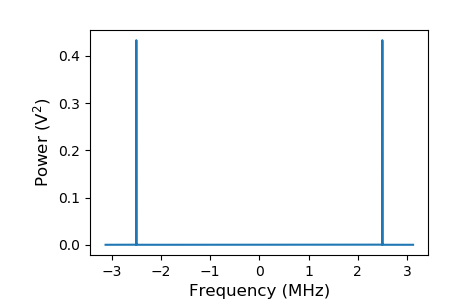
\includegraphics[width=.8\linewidth]{5-2/pow4}
	\caption{$\nu_0 = .4 \nu_s = 2.5$ MHz. Peak amplitudes at $\pm$ 2.5 MHz}
	\label{fig:NyPw4}
\end{minipage}%
\begin{minipage}{.5\textwidth}
	\centering
	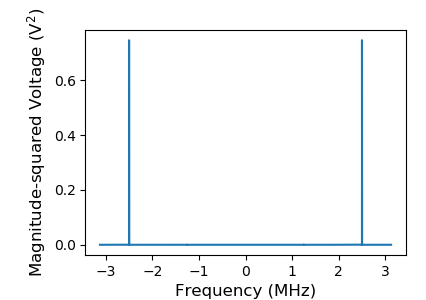
\includegraphics[width=.8\linewidth]{5-2/pow6}
	\caption{$\nu_0 = .6 \nu_s = 3.75$ MHz. Peak amplitudes at $\pm$ 2.5 MHz}
	\label{fig:NyPw6}
\end{minipage}
\end{figure}

\subsection{5.3}

The power spectra show two spikes symmetric about 0. We see them at the positive and negative of (for the non-aliased samples) the input frequency. We can consider the concept of a negative frequency in a broader context by returning to Euler's identity as recalled in the introduction.

Specifically, we calculated the voltage spectra of our samples. Since this is directly the Fourier transform, we now see real and imaginary components which are not visible in the power spectrum due to the magnitude-square operation applied to the outputs.

Differences between voltage spectra of the same signal suggest that variation in imaginary and real components are consequences of phase shifts. Taking multiple blocks of data one after the other (which loosely controls for environmental variation) allows the PicoScope to begin taking data points such that the signals do not overlap.

Power spectra are provided alongside the voltage spectra to demonstrate the power spectrum's destruction of information. The power spectrum does not change (figures \ref{fig:SyPw1}, \ref{fig:SyPw2}, and \ref{fig:SyPw3} are identical) and exhibits complete symmetry always. The voltage spectra, by contrast, are inconsistent. However, excepting noise, which seems to be influencing the patterns at the centers, the spectra are symmetric and antisymmetric in their real and imaginary components, respectively.

% ?? You probably want to put the following in the conclusion

Phase is defined with respect to some reference point; although we can discuss the phase of a single sample through its voltage spectrum, phase only becomes physically meaningful when we have multiple signals to compare. Therefore, we would find voltage spectra to be physically insightful when we are investigating multiple signals at once. Power spectra are useful for both single and simultaneous signals but, as we have seen, combined signals lead to results about the combination, and information about the individual constituents is less accessible. However, power spectra immediately provide explicit characteristics of signals, so their utility in examining individual signals is demonstrated.

% it would be kind of cool to overplot all three waveforms, in different colors...

\textcolor{red}{Come back to this section to discuss the ACF discrepancies}

``What does it mean, that the voltage spectra are complex? What do the real and imaginary
parts represent? Is the imaginary part less ‘real’ than the real part? What does it mean, for
frequencies to be negative versus positive?''

``Why might we use power spectra instead of voltage spectra, and vice versa?''

``According to the correlation theorem, the Fourier transform of the power spectrum should equal the ACF. Does it? Explain any differences.''

\

\begin{figure}
\centering
\begin{minipage}{.5\textwidth}
	\centering
	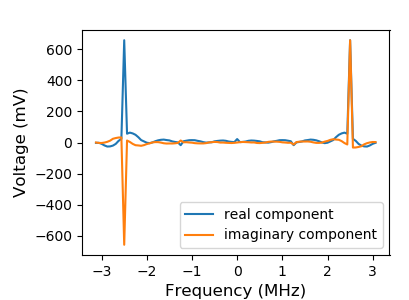
\includegraphics[width=.8\linewidth]{5-3/volt1}
	\caption{Voltage}
	\label{fig:Volt1}
\end{minipage}%
\begin{minipage}{.5\textwidth}
	\centering
	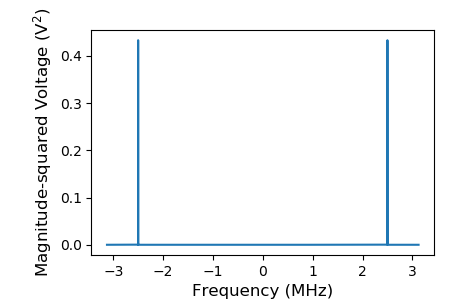
\includegraphics[width=.8\linewidth]{5-3/pow1}
	\caption{Powerish}
	\label{fig:SyPw1}
\end{minipage}
\end{figure}

\begin{figure}
\centering
\begin{minipage}{.5\textwidth}
	\centering
	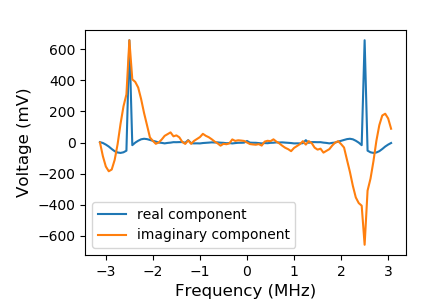
\includegraphics[width=.8\linewidth]{5-3/volt2}
	\caption{Voltage}
	\label{fig:Volt2}
\end{minipage}%
\begin{minipage}{.5\textwidth}
	\centering
	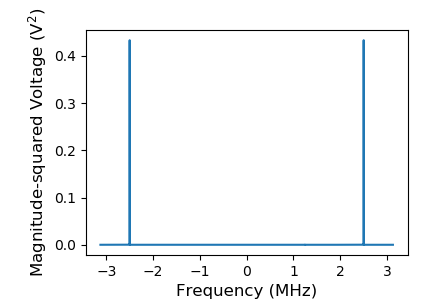
\includegraphics[width=.8\linewidth]{5-3/pow2}
	\caption{Powerish}
	\label{fig:SyPw2}
\end{minipage}
\end{figure}

\begin{figure}
\centering
\begin{minipage}{.5\textwidth}
	\centering
	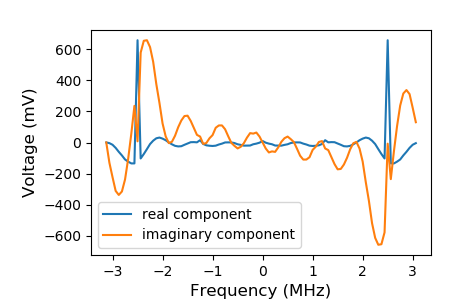
\includegraphics[width=.8\linewidth]{5-3/volt3}
	\caption{Voltage}
	\label{fig:Volt3}
\end{minipage}%
\begin{minipage}{.5\textwidth}
	\centering
	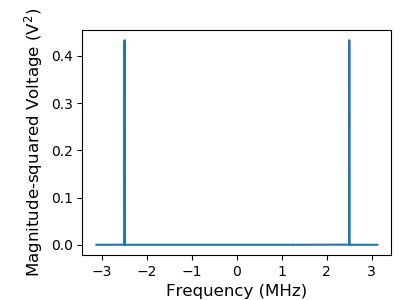
\includegraphics[width=.8\linewidth]{5-3/pow3}
	\caption{Powerishy Squishy}
	\label{fig:SyPw3}
\end{minipage}
\end{figure}

``you need to make sure dft.idft correctly infers the frequencies corresponding to each bins in your power spectrum array''

``When calculating a digital version of the correlation function, you have to worry about end effects.
Suppose you are calculating an ACF for N samples with delays ∆N ranging up to N/2. Then the
number of terms in the sum is always smaller than N because the delays spill over the edge of the
available samples.''

\textcolor{red}{How am I supposed to account for this?}

\begin{figure}
\centering
\begin{minipage}{.5\textwidth}
	\centering
	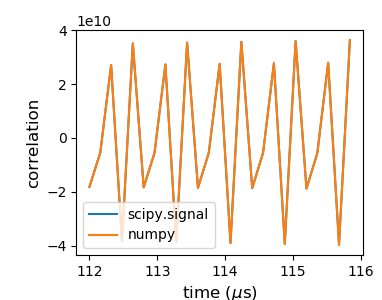
\includegraphics[width=.8\linewidth]{5-3/ACF}
	\caption{\textcolor{red}{This is supposed to be the dft/idft version}}
	\label{fig:inverse}
\end{minipage}%
\begin{minipage}{.5\textwidth}
	\centering
	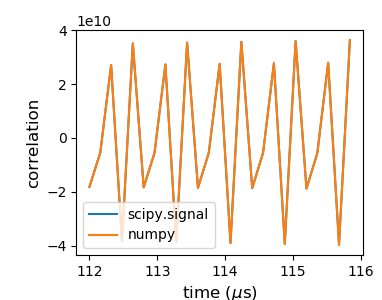
\includegraphics[width=.8\linewidth]{5-3/ACF}
	\caption{Powerish}
	\label{fig:ACF}
\end{minipage}
\end{figure}

\textcolor{red}{Differences? Probably because I did not zero out the middle}

\subsection{5.4}

\begin{figure}
\centering
\begin{minipage}{.5\textwidth}
	\centering
	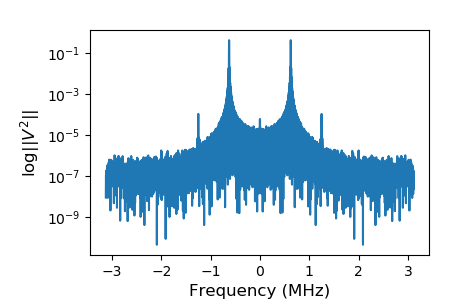
\includegraphics[width=.8\linewidth]{5-4/t1_eighth}
	\caption{$\nu_0 = .1 \nu_s = .625$ MHz}
	\label{fig:tenth_leakage}
\end{minipage}%
\begin{minipage}{.5\textwidth}
	\centering
	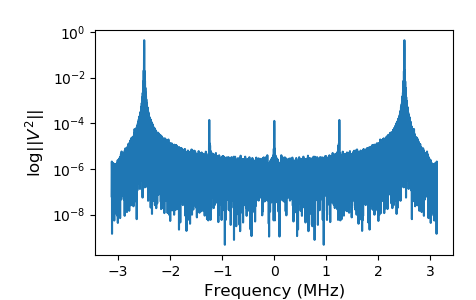
\includegraphics[width=.8\linewidth]{5-4/t4_eighth}
	\caption{$\nu_0 = .4 \nu_s = 2.5$ MHz}
	\label{fig:4tenths_leakage}
\end{minipage}
\end{figure}

\textcolor{red}{The y-axis is labeled incorrectly. We want log of square of voltage.}

Recall that spectral leakage is introduced by the finite bounds on our Fourier transforms. Why does that math correspond to these results?

\subsection{5.5}

\textcolor{red}{The separation looks pretty good so far.}

\subsection{5.6}

\begin{figure}
\centering
\begin{minipage}{.5\textwidth}
	\centering
	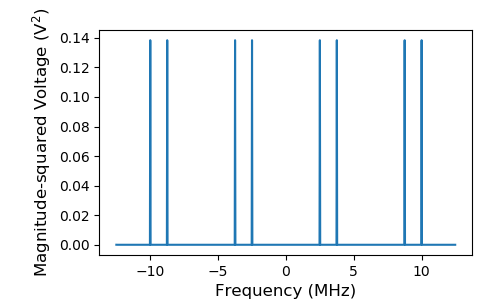
\includegraphics[width=.9\linewidth]{5-6/4window}
	\caption{$\nu_0 = .4 \nu_s = 2.5$ MHz. Fourth window.}
	\label{fig:win4}
\end{minipage}%
\begin{minipage}{.5\textwidth}
	\centering
	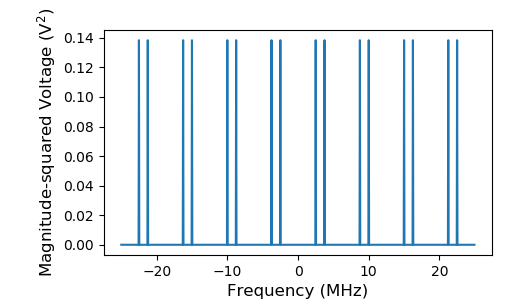
\includegraphics[width=.9\linewidth]{5-6/8window}
	\caption{Same frequency. Eighth window.}
	\label{fig:win8}
\end{minipage}
\end{figure}

\begin{figure}
\centering
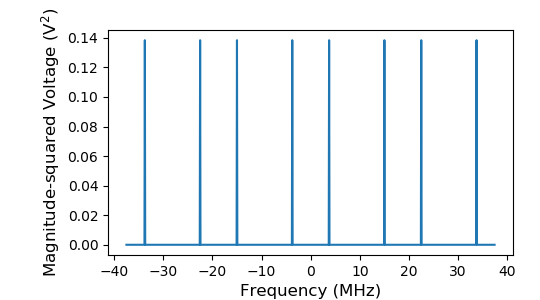
\includegraphics[width=.45\linewidth]{5-6/12window}
\caption{Same frequency. Twelfth window.}
\label{fig:win12}
\end{figure}

As we take the power spectrum out to increasing frequency ranges, we observe repetitions of the original signal which do not strictly increase in frequency, perhaps due to aliasing wrap-around.

Figures \ref{fig:win4}, \ref{fig:win8}, \ref{fig:win12} all represent power spectra for the same data and therefore also for the same input signal frequency. We continue to see pairs of spikes symmetric about the zero frequency. While the number of spike pairs increases dramatically from the fourth (figure \ref{fig:win4}) to the eighth window (\ref{fig:win8}), we see the number drop off steeply by the twelfth window. % What is your point here? I mean, it kind of feels like we're just rambling. Maybe I should cut more closely to the lab manual.

% They can't be harmonics; why else would all the spikes have the same amplitudes. And, for that matter, why do all windows show such low amplitudes? Ah, it is because the input signal (as seen on the oscilloscope) has a much lower amplitude--squaring further affects to that end.

\subsection{5.7}

First sample:

Mean = 3.899292452830189 mV
Standard deviation = 20.079642416978363 mV
Variance = 403.19203959371663 (mV)$^2$

\textcolor{red}{I am allowing the first 100 samples to contaminate. I do not know how much I should trod outside the 16000 recommendation.}

\begin{figure}
\centering
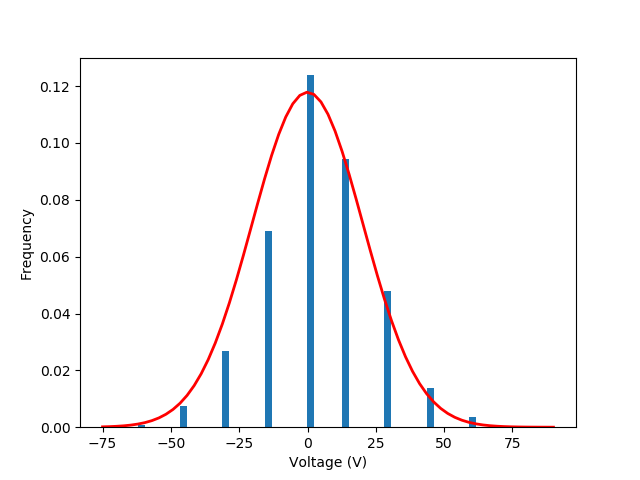
\includegraphics[width=.45\linewidth]{5-7/histo}
\caption{}
\label{fig:histogram}
\end{figure}

\begin{figure}
\centering
\begin{minipage}{.5\textwidth}
	\centering
	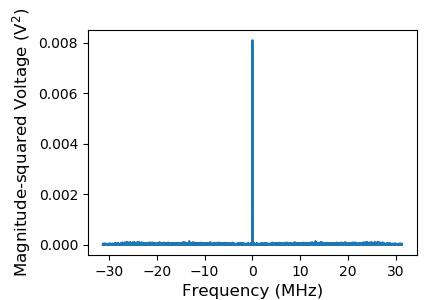
\includegraphics[width=.9\linewidth]{5-7/pow1}
	\caption{}
	\label{fig:pow1}
\end{minipage}%
\begin{minipage}{.5\textwidth}
	\centering
	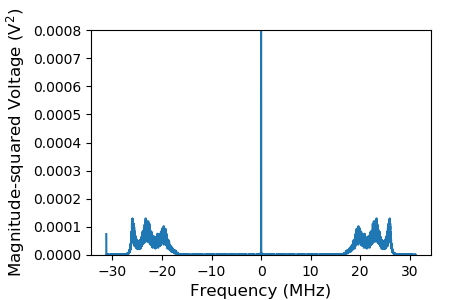
\includegraphics[width=.9\linewidth]{5-7/pow_all}
	\caption{}
	\label{fig:pow_all}
\end{minipage}
\end{figure}

\begin{figure}
\centering
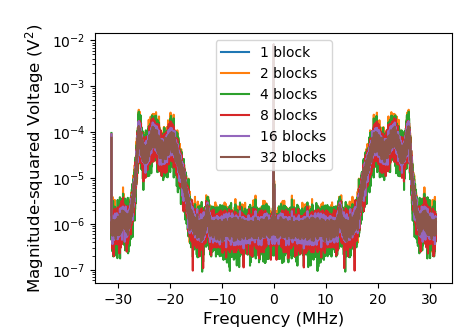
\includegraphics[width=\linewidth]{5-7/comparison}
\caption{}
\label{fig:avgs_comparison}
\end{figure}

\subsection{7.1}

Figure \ref{fig:low_display} demonstrates the principle from earlier that a sample can reconstruct a signal (e.g. via Fourier decomposition) without precise visual mimicry. In this case, each cycle of the original signal has produced a visually different sampled cycle. 

\begin{figure}
\centering
\begin{minipage}{.5\textwidth}
	\centering
	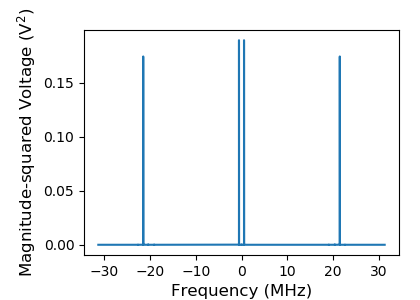
\includegraphics[width=.8\linewidth]{7-1/l_power}
	\caption{}
	\label{fig:low_pow}
\end{minipage}%
\begin{minipage}{.5\textwidth}
	\centering
	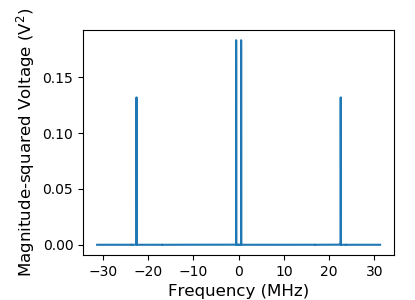
\includegraphics[width=.8\linewidth]{7-1/h_power}
	\caption{}
	\label{fig:high_pow}
\end{minipage}
\end{figure}

\begin{figure}
\centering
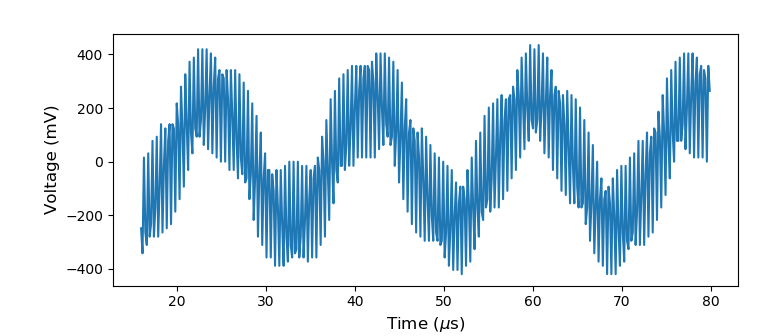
\includegraphics[width=.8\linewidth]{7-1/low_osc}
\caption{Waveform in the case where $\nu_s = 62.5$ MHz and where $\nu_{RF} = \nu{LO} - \Delta \nu = 10.45$ MHz. The largest-frequency signal is that of the sum, $2 \nu_{LO} + \Delta \nu$ = 23.1 MHz.}
\label{fig:low_display}
\end{figure}

\textcolor{red}{These figures are missing captions!}

Why do the power spectra look the way they do. Upper sideband and lower sideband.

For the upper sideband, we can see spikes at almost the difference frequency (.575 MHz $\approx$ .55 MHz). The other spikes are at 10.2 MHz? Why?

For the lower sideband, we see outer spikes at 9 MHz. The inner spikes are still at roughly the difference frequency...

\subsection{7.2}

\begin{figure}
\centering
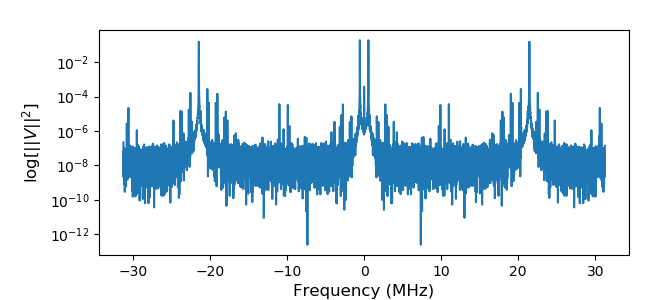
\includegraphics[width=.8\linewidth]{7-2}
\caption{}
\label{fig:intermods}
\end{figure}

\subsection{7.3}

% I really do not want to take this data, so I am deliberately leaving a more challenging analysis task for last-minute. Except it's apparently not even that challenging!

Single side band mixer is more difficult to perform.

\section{Conclusions}

\bibliographystyle{alpha}
\bibliography{sample}

\end{document}